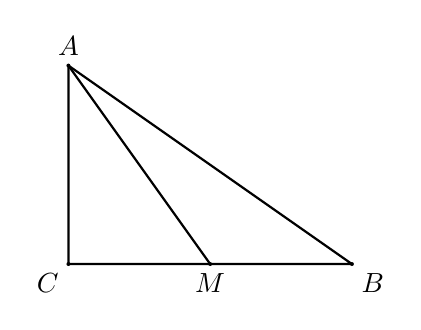
\begin{tikzpicture}[line cap=round,line join=round,scale=0.6]
% right triangle at C, with M midpoint of BC, draw AM and AB

\coordinate (C) at (0,0);
\coordinate (B) at (6,0);
\coordinate (M) at (3,0);
\coordinate (A) at (0,4.2);

% triangle edges
\draw[thick] (A)--(C)--(B)--cycle;

% median-like segment AM
\draw[thick] (A)--(M);

% points and labels
\fill (A) circle (1.2pt) node[above] {$A$};
\fill (B) circle (1.2pt) node[below right] {$B$};
\fill (C) circle (1.2pt) node[below left] {$C$};
\fill (M) circle (1.2pt) node[below] {$M$};

\end{tikzpicture}